\section{Signalklassen}
\begin{multicols}{2}
    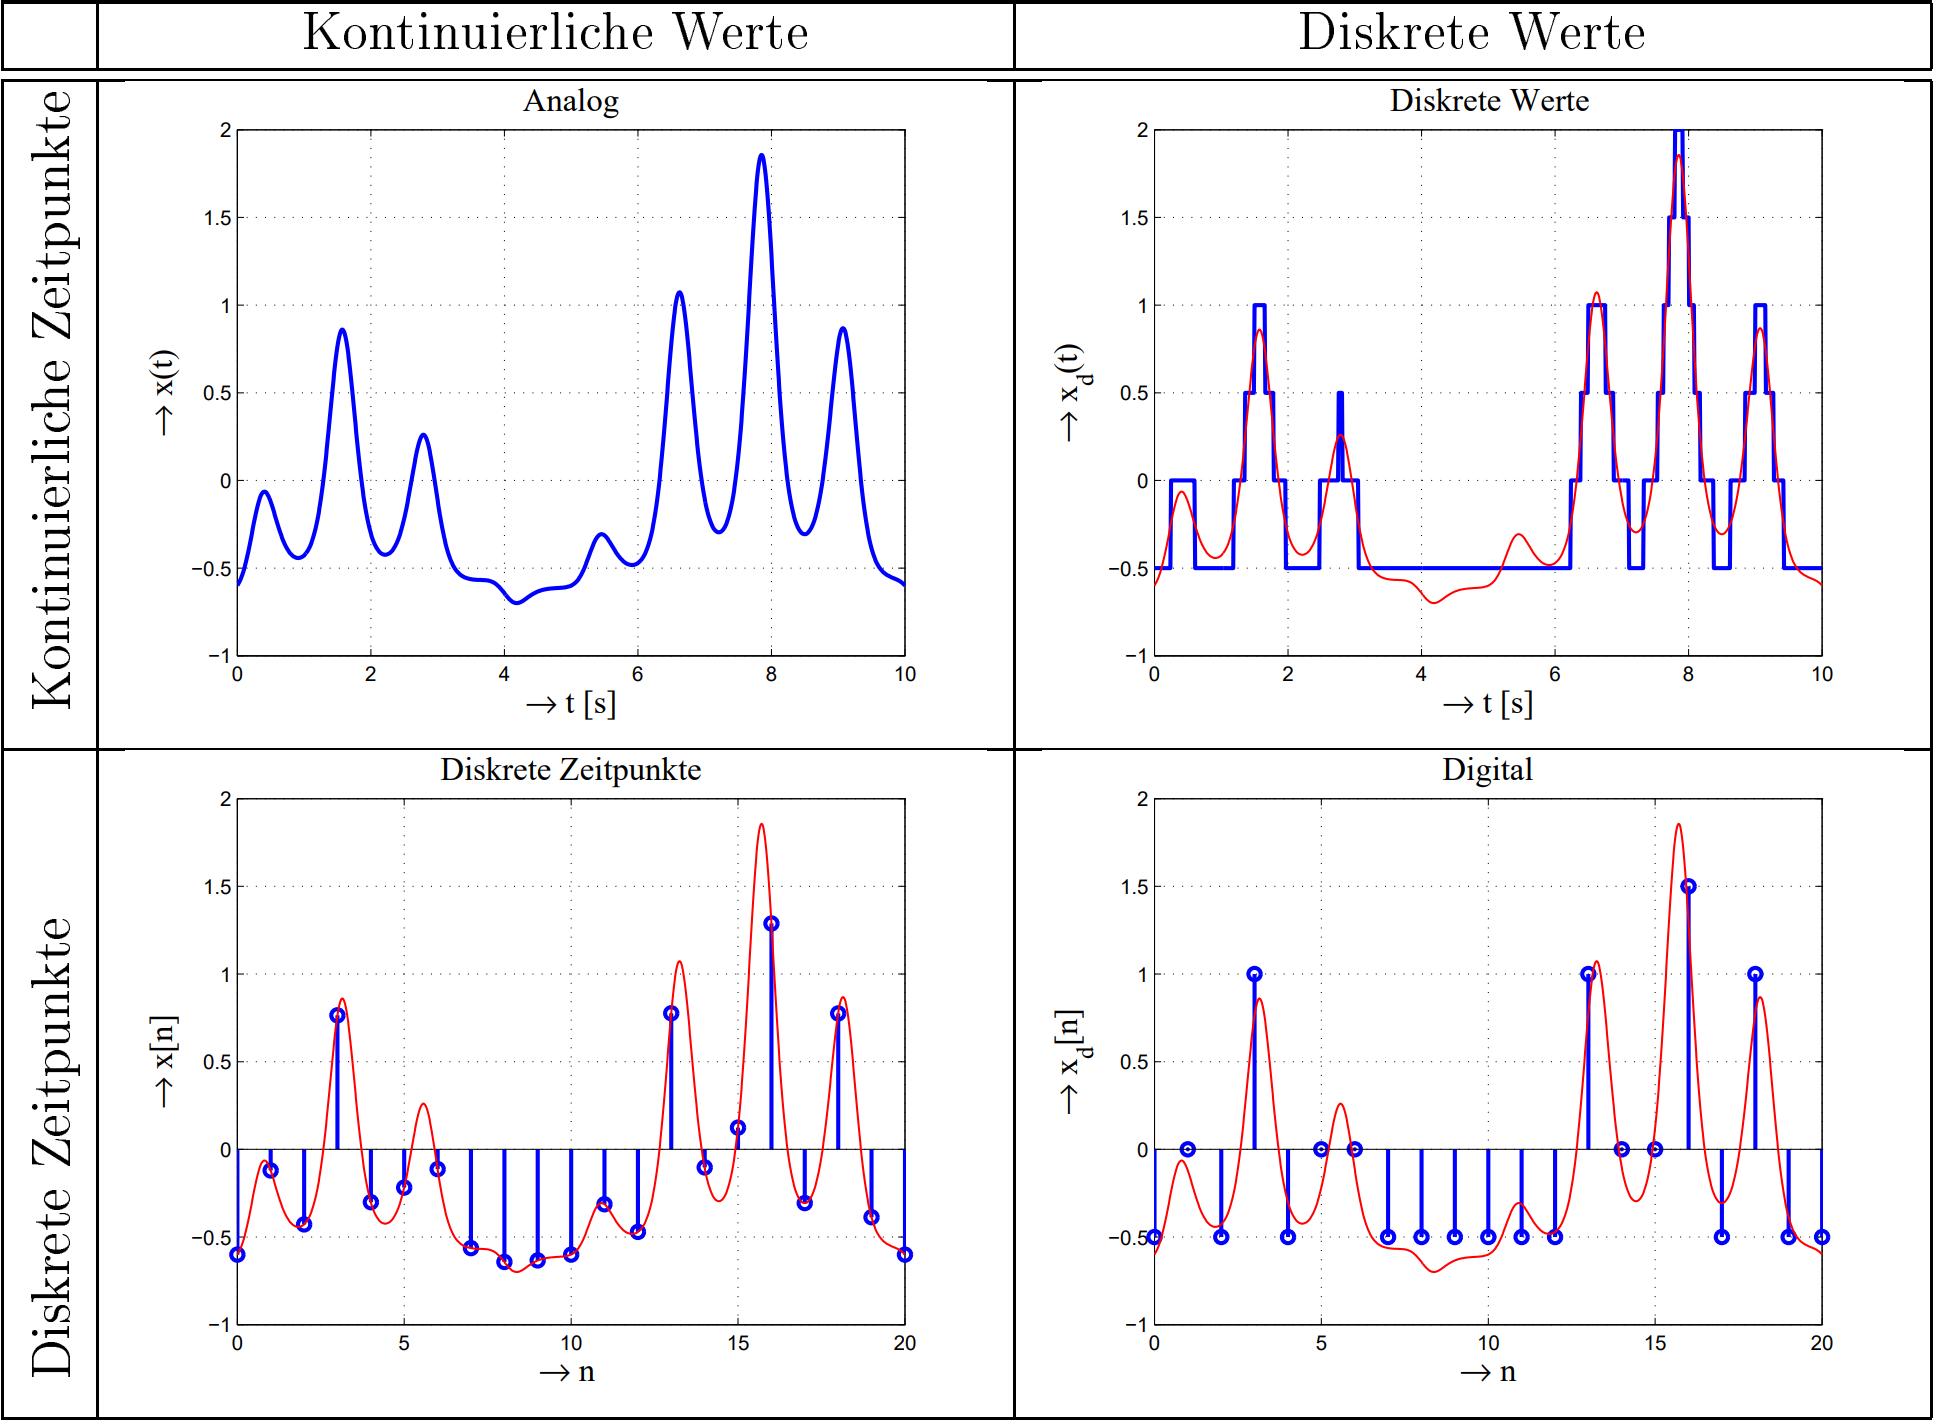
\includegraphics[width = 7cm]{include/Signalklassen/img/Signalklassen.png}
    \subsection{weitere Unterteilungen}
    \begin{tabular}{|c|c|}
        \hline
        Reellwertig $\mathbb{R}$ & Complexwertig $\mathbb{C}$ \\
        Eindimensional           & Mehrdimensional            \\
        Stochastisch             & Deterministisch            \\
        Energiesignale           & Leistungssignal            \\
        Analog                   & Digital                    \\
        Aperiodisch              & Periodisch                 \\
        \hline
    \end{tabular}
    \\[10pt]
    \begin{tabular}{|p{70pt}|p{70pt}|p{70pt}|}
        \hline
        Klasse 1            &
        Klasse 2a           &
        Klasse 2b                                                                          \\
        Energiesiegnal      & periodisches Leistungssignal & aperiodisches Leistungssignal \\
        $0 < W_n < \infty $ & $0 < P_n < \infty $          & $0 < P_n < \infty$            \\
        \hline
    \end{tabular}
\end{multicols}
